%%%%%%%%%%%%%%%%%%%%%%%%%%%%%%%%%%%%%%%%%%%%%%%%%%%%
%    Harvard Data Science Review Latex Template    %
%%%%%%%%%%%%%%%%%%%%%%%%%%%%%%%%%%%%%%%%%%%%%%%%%%%%

\documentclass[]{hdsr}

%Graphics should all go in the figs/ directory
\graphicspath{{figs/}}
\usepackage{xcolor}
\usepackage{listings}
\lstset{basicstyle=\ttfamily,
  showstringspaces=false,
  commentstyle=\color{darkred},
  keywordstyle=\color{blue}
}

\begin{document}

% Larger bottom margin for the first page
\newgeometry{bottom=1.5in}

% Editorial staff will replace the following values:
% 1. Volume number
% 2. Issue number
% 3. Article DOI
% e.g. for Volume 2, Issue 3, DOI 12.345:
% \volumeheader{2}{3}{12.345}
\volumeheader{0}{0}{00.000}



\begin{center}

  \title{A Very Enticing Title}
  \maketitle

  % Start page numbering on second page. Must appear *after* \maketitle
  \thispagestyle{empty}
  
  \vspace*{.2in}

  % Authors and Affiliations
  \begin{tabular}{cc}
    First Author\upstairs{\affilone,*}, Second Author\upstairs{\affilone}, Third Author\upstairs{\affilthree}
   \\[0.25ex]
   {\small \upstairs{\affilone} Affiliation One} \\
   {\small \upstairs{\affiltwo} Affiliation Two} \\
   {\small \upstairs{\affilthree} Affiliation Three} \\
  \end{tabular}
  
  % Replace with corresponding author email address
  \emails{
    \upstairs{*}correspondingauthor@example.edu 
    }
  \vspace*{0.4in}

\begin{abstract}
The abstract should be no more than 250 words.
\end{abstract}
\end{center}

\vspace*{0.15in}
\hspace{10pt}
  \small	
  \textbf{\textit{Keywords: }} {up, to, six, keywords}
  
\copyrightnotice

\section*{Media Summary}
The Media Summary should be written in plain language to highlight the key messages of
the article, in ways that can be understood by the general public and cited by the media 
directly and accurately.  It therefore should avoid technical terms or language designed for
academic communications. It should not exceed 400 words, and more succinct, the better.

\section{An Informative Section Title}
\label{sec1}
Because we use section titles in a pull-down menu for the online version as signposts, please use as specific and informative titles as possible. Avoid generic section titles such as ``methods,'' ``data,'' and ``results''. Such titles are common in certain technical journals, but they do not work well for HDSR, which aims to publish ``everything data science and data science for everyone". Try to use titles that will make readers (and you!) think that ``Hmmm, that sounds interesting'' or ``Hmmm, that's unexpected and I better to take a look.''   The same goes with the article title, and indeed the entire article.  Considering you are not writing a technical article, but rather telling a data science story with layered plots, an enticing flow, and a memorable punch line. That is, an article you want to read, and will walk away feeling ``Wow, that was inspiring -- I never thought about that!'' 

\begin{equation}
    i\hbar \frac{\partial \Psi}{\partial t} = -\frac{\hbar^2}{2m}
\frac{\partial^2 \Psi}{\partial x^2} + V \Psi
\end{equation}


\subsection{Subsection}

Building upon previous work by \citet{2020.03.27.20043752},  dolor sit amet, consectetur adipiscing elit. Pellentesque id massa vulputate, tristique mi id, imperdiet mi.

\section{Section Title}
Lorem ipsum dolor sit amet, consectetur adipiscing elit. Pellentesque id massa vulputate, tristique mi id, imperdiet mi. Mauris id ante ac lacus mollis sagittis. Sed imperdiet nibh id eros malesuada, at fermentum urna mollis. Sed id elit eu arcu varius tempor tincidunt in orci. Nullam accumsan diam vitae nibh fermentum, nec facilisis leo pulvinar. Ut condimentum nisl in orci euismod mattis. Fusce at mauris augue. 


% These commands need to appear at the point where you want
% the first page to end.
\restoregeometry
\newgeometry{bottom=0.5in}

\section{Section Title}
Lorem ipsum dolor sit amet, consectetur adipiscing elit. Pellentesque id massa vulputate, tristique mi id, imperdiet mi. Mauris id ante ac lacus mollis sagittis. Sed imperdiet nibh id eros malesuada, at fermentum urna mollis. 

\begin{equation}
-\frac{\hbar^2}{2m} \frac{d^2 \psi}{dx^2} + V\psi = E\psi\\
\end{equation}


Sed id elit eu arcu varius tempor tincidunt in orci. Nullam accumsan diam vitae nibh fermentum, nec facilisis leo pulvinar. Ut condimentum nisl in orci euismod mattis. Fusce at mauris augue. 

% 1. When figure position is crucial, use the [H] tag 
%    to enforce absolute positioning
% 2. Image files should be referenced without file extension
\begin{figure}[H]
    \centering
    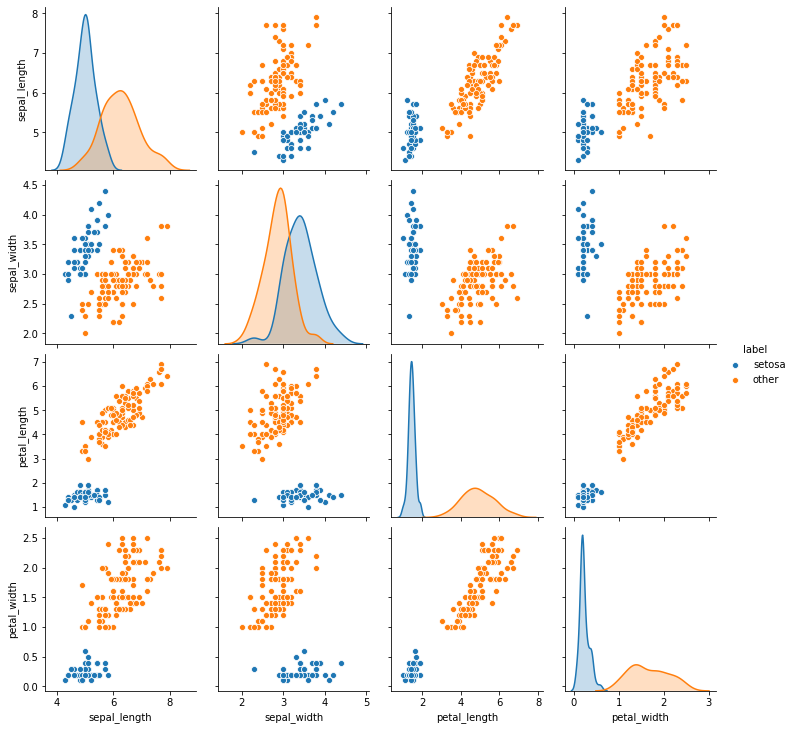
\includegraphics[scale=0.35]{iris_pairs} \\
    \caption{This is an example figure}
    \label{fig:my_label}
\end{figure}


\subsection*{Disclosure Statement}
The authors have no conflicts of interest to declare.

\subsection*{Acknowledgments}
Lorem ipsum dolor sit amet, consectetur adipiscing elit. Pellentesque id massa vulputate, tristique mi id, imperdiet mi. Mauris id ante ac lacus mollis sagittis. Sed imperdiet nibh id eros malesuada, at fermentum urna mollis. Sed id elit eu arcu varius tempor tincidunt in orci. Nullam accumsan diam vitae nibh fermentum, nec facilisis leo pulvinar. Ut condimentum nisl in orci euismod mattis. Fusce at mauris augue. 
 
\subsection*{Contributions}
Lorem ipsum dolor sit amet, consectetur adipiscing elit. Pellentesque id massa vulputate, tristique mi id, imperdiet mi. Mauris id ante ac lacus mollis sagittis. Sed imperdiet nibh id eros malesuada, at fermentum urna mollis. Sed id elit eu arcu varius tempor tincidunt in orci. Nullam accumsan diam vitae nibh fermentum, nec facilisis leo pulvinar. Ut condimentum nisl in orci euismod mattis. Fusce at mauris augue. 


%Begin appendix section(s)
\appendix

% Add appendices here:
\section{Title}
\label{appendix-customize-this-label}
Lorem ipsum dolor sit amet, consectetur adipiscing elit. Pellentesque id massa vulputate, tristique mi id, imperdiet mi. Mauris id ante ac lacus mollis sagittis. Sed imperdiet nibh id eros malesuada, at fermentum urna mollis. Sed id elit eu arcu varius tempor tincidunt in orci. 

\begin{equation}
e^{i\theta} = \cos \theta + i\sin \theta
\end{equation}

Nullam accumsan diam vitae nibh fermentum, nec facilisis leo pulvinar. Ut condimentum nisl in orci euismod mattis. Fusce at mauris augue. 


% All references should be stored in the file "references.bib"
% Please do not modify anything below this line.
\printbibliography


\end{document}
